\documentclass[11pt,a4paper]{report}

% ── Essential Packages ──────────────────────────────────────────
\usepackage[utf8]{inputenc}
\usepackage[T1]{fontenc}
\usepackage{lmodern}
\usepackage[a4paper,top=25mm,bottom=25mm,left=25mm,right=22mm,headheight=14pt]{geometry}
\usepackage{graphicx}
\usepackage{amsmath,amssymb,amsfonts}
\usepackage{booktabs}
\usepackage{tabularx}
\usepackage{longtable}
\usepackage{array}
\usepackage{multirow}
\usepackage{xcolor}
\usepackage{fancyhdr}
\usepackage{titlesec}
\usepackage{tikz}
\usetikzlibrary{shapes.geometric,arrows.meta,positioning,calc,fit,backgrounds}
\usepackage{tcolorbox}
\tcbuselibrary{skins,breakable}
\usepackage[colorlinks=true,linkcolor=black,citecolor=black,urlcolor=blue]{hyperref}

% ── Color Definitions ───────────────────────────────────────────
\definecolor{upesred}{RGB}{199,91,57}
\definecolor{agrigreen}{RGB}{27,67,50}
\definecolor{headerblue}{RGB}{0,51,102}
\definecolor{boxbg}{RGB}{245,248,252}

% ── Typography & Chapter Formatting ─────────────────────────────
\titleformat{\chapter}[display]
  {\normalfont\bfseries\Large}
  {\MakeUppercase{\chaptertitlename}\ \thechapter}{4pt}{\Huge\bfseries}
\titlespacing*{\chapter}{0pt}{-10pt}{20pt}

\titleformat{\section}
  {\normalfont\Large\bfseries}{\thesection}{1em}{}
\titleformat{\subsection}
  {\normalfont\large\bfseries}{\thesubsection}{1em}{}

% ── Header & Footer Setup ───────────────────────────────────────
\pagestyle{fancy}
\fancyhf{}
\fancyhead[L]{\textit{Project Report}}
\fancyhead[R]{\textit{KissanVision}}
\fancyfoot[C]{Page \thepage}
\renewcommand{\headrulewidth}{0.4pt}
\renewcommand{\footrulewidth}{0pt}

% Style for plain pages (chapter starts)
\fancypagestyle{plain}{
  \fancyhf{}
  \fancyhead[L]{\textit{Project Report}}
  \fancyhead[R]{\textit{KissanVision}}
  \fancyfoot[C]{Page \thepage}
  \renewcommand{\headrulewidth}{0.4pt}
}

% ── Custom Callout Boxes ────────────────────────────────────────
\newtcolorbox{problemstatementbox}{
  colback=boxbg,
  colframe=headerblue,
  coltitle=white,
  fonttitle=\bfseries\sffamily\small,
  title=Problem Statement,
  arc=2mm,
  boxrule=1pt,
  left=10pt,right=10pt,top=8pt,bottom=8pt,
  breakable
}

\newtcolorbox{algorithmbox}[1]{
  colback=white,
  colframe=agrigreen,
  coltitle=white,
  fonttitle=\bfseries\sffamily\small,
  title={#1},
  arc=2mm,
  boxrule=1pt,
  left=10pt,right=10pt,top=8pt,bottom=8pt,
  breakable
}

% ── Document Starts ─────────────────────────────────────────────
\begin{document}

% ================================================================
% COVER / TITLE PAGE
% ================================================================
\begin{titlepage}
\centering
\vspace*{5mm}

{\Large \textbf{Project Report}}\\[3mm]
{\normalsize on}\\[6mm]

{\Huge \textbf{KissanVision}}\\[4mm]
{\Large \textit{An AI-Powered Crop Yield Prediction and Agronomic Decision Intelligence Platform for Indian Agriculture}}\\[10mm]

{\normalsize Submitted in partial fulfilment of the requirements for the award of the degree of}\\[3mm]
{\Large \textbf{Bachelor of Technology}}\\[2mm]
{\normalsize in}\\[2mm]
{\large \textbf{Computer Science and Engineering}}\\[1mm]
{\normalsize with specialization in \textbf{Data Science}}\\[10mm]

\textbf{Submitted by}\\[4mm]
\begin{tabular}{|l|c|l|c|}
\hline
\textbf{Specialization} & \textbf{SAP ID} & \textbf{Name} & \textbf{Batch} \\
\hline
Data Science & 500120442 & Animesh Gupta & 02 \\
Data Science & 500120443 & Nilay & 01 \\
Data Science & 500119637 & Amit Kumar & 01 \\
\hline
\end{tabular}\\[10mm]

{\normalsize Under the guidance of}\\[2mm]
{\large \textbf{Dr. Archana Kumari}}\\[1mm]
{\normalsize \textit{Project Mentor}}\\[10mm]


\begin{tikzpicture}
  \node[draw=upesred, rounded corners=3pt, line width=1.5pt, inner sep=6pt] {
    {\Huge \textbf{\color{upesred}UPES}}
  };
\end{tikzpicture}\\[2mm]
{\footnotesize \textbf{UNIVERSITY OF THE FUTURE}}\\[4mm]

{\normalsize \textbf{School of Computer Science}}\\[1mm]
{\large \textbf{UNIVERSITY OF PETROLEUM \& ENERGY STUDIES}}\\[1mm]
{\normalsize DEHRADUN -- 248007, Uttarakhand}\\[6mm]

{\large \textbf{October 2026 \quad\textbar\quad Version 3.2.0}}

\end{titlepage}

% ================================================================
% FRONT MATTER
% ================================================================
\pagenumbering{roman}
\setcounter{page}{2}

% ── Candidates' Declaration ─────────────────────────────────────
\chapter*{Candidates' Declaration}
\addcontentsline{toc}{chapter}{Candidates' Declaration}

We hereby declare that the project work presented in this report, entitled \textbf{``KissanVision: An AI-Powered Crop Yield Prediction and Agronomic Decision Intelligence Platform for Indian Agriculture''}, submitted in partial fulfilment of the requirements for the award of the degree of \textbf{Bachelor of Technology in Computer Science and Engineering with specialization in Data Science}, at the School of Computer Science, University of Petroleum and Energy Studies, Dehradun, is an authentic record of our own work, carried out from August 2026 to October 2026 under the guidance of \textbf{Dr. Archana Kumari}.

The work in this report has not been submitted by us for the award of any other degree or diploma. Wherever we have used the ideas, words or data of other people, we have named the source in the references.\\[25mm]

\noindent
\begin{tabular*}{\textwidth}{@{\extracolsep{\fill}}ccc}
\rule{45mm}{0.5pt} & \rule{45mm}{0.5pt} & \rule{45mm}{0.5pt} \\
\textbf{Animesh Gupta} & \textbf{Nilay} & \textbf{Amit Kumar} \\
SAP ID: 500120442 & SAP ID: 500120443 & SAP ID: 500119637
\end{tabular*}

\vspace{25mm}
\noindent
\textbf{Date:} 13 October 2026 (Tuesday)\\
\textbf{Place:} Dehradun

\newpage

% ── Certificate ─────────────────────────────────────────────────
\chapter*{Certificate}
\addcontentsline{toc}{chapter}{Certificate}

This is to certify that the project report entitled \textbf{``KissanVision: An AI-Powered Crop Yield Prediction and Agronomic Decision Intelligence Platform for Indian Agriculture''}, submitted by \textbf{Animesh Gupta} (SAP ID 500120442), \textbf{Nilay} (SAP ID 500120443), and \textbf{Amit Kumar} (SAP ID 500119637) in partial fulfilment of the requirements for the award of the degree of \textbf{Bachelor of Technology in Computer Science and Engineering with specialization in Data Science}, is a record of the work carried out by them under my supervision.

To the best of my knowledge, the work in this report has not been submitted elsewhere for the award of any other degree or diploma.\\[35mm]

\noindent
\rule{60mm}{0.5pt}\\
\textbf{Dr. Archana Kumari}\\
\textit{Project Mentor}\\
School of Computer Science, UPES, Dehradun\\[10mm]
\textbf{Date:} \rule{40mm}{0.5pt}

\newpage

% ── Acknowledgement ─────────────────────────────────────────────
\chapter*{Acknowledgement}
\addcontentsline{toc}{chapter}{Acknowledgement}

We are deeply grateful to our project mentor, \textbf{Dr. Archana Kumari}, for guiding us from the very first conceptualization to this final report. Every milestone review pushed us to ask a harder question: not only \textit{``does the machine learning model converge with high $R^2$?''}, but also \textit{``would a smallholder farmer in Vidarbha or an extension agronomist in Punjab understand why this prediction was made and trust its recommendations?''}. That single guiding question shaped almost every design choice in KissanVision.

We thank the School of Computer Science, University of Petroleum and Energy Studies, Dehradun, for providing the academic infrastructure, laboratories, research guidance, and computational facilities to work on a real-world societal challenge.

We are indebted to the open-source community and global scientific repositories. This project stands on Python, XGBoost, scikit-learn, SHAP, FastAPI, Streamlit, Plotly, pandas, and the public climatology repositories of NASA POWER and Open-Meteo ECMWF. We also thank the Ministry of Agriculture and Farmers Welfare and the Directorate of Economics and Statistics for maintaining open agricultural data. The methodologies established in cited research saved us from many false turns.

Finally, we thank our families and friends for their enduring patience during the long evenings and intensive development sprints that a full-scale project like this demands.\\[15mm]

\noindent
\textbf{Animesh Gupta \quad\textbar\quad Nilay \quad\textbar\quad Amit Kumar}

\newpage

% ── Abstract ────────────────────────────────────────────────────
\chapter*{Abstract}
\addcontentsline{toc}{chapter}{Abstract}

Agriculture forms the backbone of India’s rural economy, engaging over 43\% of the nation's workforce and contributing nearly 18\% to Gross Value Added (GVA). Yet, agricultural planning remains heavily vulnerable to monsoon vagaries, climate shifts, uncalibrated fertilizer application, and erratic market dynamics. While millions of historical crop, soil, and meteorological records exist across state repositories, smallholder farmers and district extension workers lack accessible, trustworthy, and actionable intelligence to forecast harvest productivity before sowing. Furthermore, prevailing machine learning systems in research operate as opaque black boxes, providing point estimates without agronomic provenance, weather-scenario sensitivity, or local explainability.

\textbf{KissanVision} is our solution to close this critical divide. It is a production-grade, full-stack decision intelligence platform that integrates 50,000 real Indian district-level records spanning 33 States/UTs, 15 major crops, and 6 cropping seasons with live climatology, farmer-level input overrides, and game-theoretic explainability. Rather than treating yield prediction in isolation, KissanVision unifies:
\begin{enumerate}
  \item \textbf{A Tuned XGBoost Regression Engine} achieving a validated $R^2$ of \textbf{0.9165}, an RMSE of \textbf{12.07 Quintals/Hectare (q/ha)}, and an MAE of \textbf{5.57 q/ha} on held-out stratified test samples across 59 engineered features;
  \item \textbf{Dual Meteorological Modalities}: a historical 3-year baseline powered by NASA POWER Agroclimatology alongside a next-season forecast engine powered by Open-Meteo ECMWF SEAS5 51-member ensemble spanning a 180-day seasonal horizon;
  \item \textbf{Farmer Personalization Overrides}: allowing growers to substitute regional defaults with actual farm-measured irrigation coverage percentage and NPK consumption (kg/ha), tracked via provenance badges;
  \item \textbf{Agro-Climatic Stress Early Warning}: evaluating real-time temperatures, moisture, and rainfall against ICAR (Indian Council of Agricultural Research) thresholds to flag drought, flood, heatwave, and humidity disease risks across all 33 states;
  \item \textbf{Game-Theoretic Local Interpretability}: implementing SHAP (SHapley Additive exPlanations) TreeExplainer to break down every single prediction into baseline expected yield plus individual feature contributions in waterfall and ranking visualizations;
  \item \textbf{Multi-Channel Serving}: deploying an interactive Streamlit agronomy dashboard, a responsive HTML5/CSS3/JavaScript web interface, and an enterprise FastAPI REST microservice with 15 documented OpenAPI endpoints operating with sub-50ms inference latency.
\end{enumerate}

Across our benchmark test suite, all unit, API, integration, and contract tests pass with 100\% compliance. On a standard laptop, cold-start inference completes in under 45 ms and cached weather responses return in under 3 ms, providing a scalable, free-forever, and auditable digital public infrastructure for Indian farmers.\\[8mm]

\noindent
\textbf{Keywords:} Decision Intelligence, Precision Agriculture, Crop Yield Prediction, XGBoost, SHAP Explainability, NASA POWER, Open-Meteo ECMWF SEAS5, Agro-Climatology, Farmer Personalization, FastAPI.

\newpage

% ── Version History ─────────────────────────────────────────────
\chapter*{Version History}
\addcontentsline{toc}{chapter}{Version History}

This report went through three formal versions. Each version was dated on a working day and shared with our mentor, Dr. Archana Kumari, for review. Version 3.2.0 is the final version presented in this document.\\[4mm]

\noindent
\begin{tabularx}{\textwidth}{|c|c|X|X|c|}
\hline
\textbf{Ver.} & \textbf{Date} & \textbf{What Changed} & \textbf{Reason for Change} & \textbf{Mentor Sign.} \\
\hline
1.0 & Wed, 7 Oct 2026 & First draft of Chapters 1 to 3: introduction, agrarian background study, and requirement analysis with feasibility. & First draft, shared to agree on the research scope and engineering methodology. & \\
\hline
2.0 & Fri, 9 Oct 2026 & Added Chapters 4 to 6: multi-layer architecture, 50K-row XGBoost pipeline, dual weather integration, SHAP explainability, and test suite. & Expanding specification to encompass working codebase, verified metrics, and UI screens. & \\
\hline
3.2.0 & Mon, 12 Oct 2026 & Final submission version. Added Chapter 7, abstract, and bibliography. Attached complete Software Requirements Specification (Part II), analysis models, and test logs. & Final academic submission conforming to UPES B.Tech Data Science guidelines. & \\
\hline
\end{tabularx}

\vspace{10mm}
\noindent
\textbf{\large How to read this report}
\begin{itemize}
  \item \textbf{Part I (Chapters 1 to 7)} is the project report. It tells the story of the project: the agricultural problem, what existing research has established, the system architecture, how we implemented and validated the models, and empirical findings.
  \item \textbf{Part II} is the complete Software Requirements Specification (SRS). It is the formal, detailed list of what the system must do conforming to IEEE Std 830-1998 and ISO/IEC/IEEE 29148:2018.
  \item \textbf{Agricultural Units}: Crop yield is measured in standard Indian agricultural units: \textbf{Quintals per Hectare (q/ha)}, where $1\text{ Quintal} = 100\text{ kg}$ and $1\text{ Hectare} = 10,000\text{ m}^2$. Land area is in Hectares (ha). Fertilizer is in kilograms per hectare (kg/ha). Rainfall is in millimeters (mm).
  \item Numbers in square brackets, for example [4], point to the formal bibliography at the end of Part I. Abbreviations like SHAP, NPK, ICAR, and OHE are defined in Appendix A.
\end{itemize}

\newpage

% ── Table of Contents & Lists ───────────────────────────────────
\tableofcontents
\newpage
\listoffigures
\newpage
\listoftables
\newpage

% ================================================================
% PART I: PROJECT REPORT
% ================================================================
\pagenumbering{arabic}
\setcounter{page}{1}

\part{Project Report}

% ── CHAPTER 1 ───────────────────────────────────────────────────
\chapter{Introduction}

\section{Background and Problem}
Indian agriculture accounts for approximately 18.3\% of India's national Gross Value Added (GVA) and provides livelihood to over 58\% of rural households [1]. Spanning 33 States and Union Territories across diverse agro-ecological zones---from the fertile alluvial plains of the Indo-Gangetic basin to the semi-arid Deccan plateau---farming in India is predominantly carried out by small and marginal farmers with landholdings under 2 hectares [2].

Despite tremendous technological strides in satellite remote sensing and crop genetics, Indian farming remains precarious. Over 50\% of net cultivated area in India is rainfed, rendering harvests acutely vulnerable to southwest monsoon variability, dry spells, heat stress during grain filling, and unseasonal cloudbursts [3]. Concurrently, imbalanced fertilizer application---characterized by an over-reliance on subsidized urea at the expense of balanced NPK (Nitrogen, Phosphorus, Potassium) ratios---depletes soil health and yields diminishing returns [4].

While governmental agencies and research institutes maintain extensive district-level records on crop acreages, historic harvests, and state-level input averages, this wealth of data remains functionally isolated in static statistical abstracts. When an Indian farmer plans their seasonal sowing, decisions regarding crop choice, expected yields, and input allocations are predominantly made from ancestral intuition or informal advice from local input dealers. Traditional agricultural extension mechanisms (e.g., Krishi Vigyan Kendras) face severe human resource constraints, with the farmer-to-extension worker ratio exceeding 1,160:1 [5]. Large commercial digital systems remain opaque black boxes.

\begin{problemstatementbox}
Smallholder farmers and agricultural stakeholders lack an accessible, transparent, and climate-adaptive digital decision system that predicts harvest yields (Quintals/Hectare) with proven precision, bridges historical climatology with seasonal weather forecasts, allows farmers to override regional defaults with their actual farm-measured inputs, flags agro-climatic stress risks, and provides game-theoretic local explainability (SHAP) for every prediction without requiring paid subscriptions.
\end{problemstatementbox}

\section{Objectives}
KissanVision was engineered to achieve nine clear, measurable objectives:
\begin{enumerate}
  \item \textbf{Unify Multi-Source Agronomic Data}: Ingest, clean, and enrich 50,000 real district records across 33 states, 15 crops, and 6 seasons, converting production to Quintals/Hectare.
  \item \textbf{High-Precision Regression Modeling}: Train and tune an XGBoost regression model with 5-fold cross-validation achieving validated test $R^2 \ge 0.90$.
  \item \textbf{Dual Climatological Modalities}: Integrate historical 3-year NASA POWER climatology alongside Open-Meteo ECMWF SEAS5 51-member ensemble seasonal forecasts.
  \item \textbf{Empower Farmer Overrides}: Enable growers to substitute regional defaults with actual farm-measured irrigation coverage percentage and NPK consumption (kg/ha) with visual source badges.
  \item \textbf{Agro-Climatic Stress Early Warning}: Detect drought, flood, heatwave, and humidity disease risks using validated ICAR thresholds across all 33 states.
  \item \textbf{Local Game-Theoretic Explainability}: Compute exact SHAP values for every prediction, rendering interactive waterfall attribution diagrams.
  \item \textbf{Multi-Channel Serving}: Deliver an interactive Streamlit agronomy dashboard, a responsive modern web UI, and an enterprise FastAPI REST service with 15 documented endpoints.
  \item \textbf{Zero Cost Barrier}: Construct the entire technology pipeline utilizing 100\% free and open-source components with zero paid API keys.
  \item \textbf{High Operational Speed}: Deliver sub-50ms inference latency with 100\% automated test suite coverage.
\end{enumerate}

\section{Scope}
\textbf{In scope.} 15 major Indian foodgrains, pulses, oilseeds, and cash crops (Rice, Wheat, Maize, Potato, Onion, Groundnut, Gram, Dry Chillies, Rapeseed \& Mustard, Jowar, Sunflower, Sesamum, Moong, Urad, Arhar/Tur) across all 33 Indian States and Union Territories and 6 cropping seasons. NASA POWER climatology, Open-Meteo ECMWF SEAS5 ensemble, Agricultural Census irrigation data, and Ministry of Chemicals \& Fertilizers NPK consumption.

\textbf{Out of scope.} Spot mandi commodity trading, automated crop insurance claim payouts, and drone-based multispectral NDVI raster processing at 10-meter pixel resolution.

\section{Our Contribution}
The individual mathematical algorithms are established in scientific literature. What is genuinely innovative is how they are synthesized for Indian agriculture:
\begin{itemize}
  \item \textbf{A Closed Transparent Agronomic Loop}: Real district records, 59-feature encoding, XGBoost regression, dual-mode meteorology, farmer overrides, and live SHAP waterfall decomposition unified in one runtime;
  \item \textbf{Honest Metrics on Real Data}: Trained and tested on 50,000 authentic district-level records preserving real agrarian variance ($R^2 = 0.9165$, RMSE = 12.07 q/ha) rather than misleading synthetic overfits;
  \item \textbf{Ensemble Seasonal Climate Forecasting}: Dynamically integrating Open-Meteo's ECMWF SEAS5 51-member ensemble forecast to estimate next-season yields before sowing begins;
  \item \textbf{Provenance-Aware Personalization}: Permitting instant farm-level overrides of irrigation and fertilizer while visibly tagging data provenance on screen;
  \item \textbf{Zero-Cost Enterprise-Ready Stack}: Multi-channel delivery via FastAPI REST microservice, Streamlit analytical dashboard, and modern web UI requiring zero recurring cloud fees.
\end{itemize}

\section{Organisation of the Report}
Chapter 2 reviews related agronomic and ML literature, Chapter 3 details requirements and feasibility, Chapter 4 presents system design, Chapter 5 outlines implementation, Chapter 6 discusses testing and empirical results, and Chapter 7 concludes the report. Part II provides the complete Software Requirements Specification (SRS).

% ── CHAPTER 2 ───────────────────────────────────────────────────
\chapter{Background Study}

\section{Analytics and Machine Learning in Agriculture That People Trust}
Davenport and Harris demonstrated that analytics delivers ROI only when operational stakeholders act upon recommendations [7]. For high-stakes decisions like agricultural sowing---where an erroneous choice can plunge a farming household into debt---Rudin argues that when an interpretable or thoroughly explained model performs comparably to a black box, the interpretable approach must be used [8]. Ribeiro et al. [9] and Lundberg \& Lee [10] proved that end users trust models when they can inspect why a prediction was made. KissanVision implements game-theoretic SHAP local explanations to ensure every output is fully auditable.

\section{Methods We Build On}
Table 2.1 summarizes the foundational concepts from literature that inform the architecture of KissanVision.

\begin{table}[htbp]
\centering
\small
\caption{Ideas from the agronomic and ML literature and how KissanVision uses them}
\begin{tabularx}{\textwidth}{lXX}
\toprule
\textbf{Area} & \textbf{Scientific Finding / Reference} & \textbf{What KissanVision Took} \\
\midrule
\textbf{Gradient Boosting} & XGBoost consistently outperforms deep nets on tabular data, handling sparsity and non-linear interactions [11]. & Tuned \texttt{XGBRegressor} over 59 features, optimized via 3-fold GridSearchCV. \\
\addlinespace
\textbf{Local Explainability} & Shapley values provide mathematically unique, additive feature attribution fulfilling efficiency and symmetry axioms [10]. & \texttt{shap.TreeExplainer} in runtime; waterfall plots showing baseline + sum(SHAP) = yield. \\
\addlinespace
\textbf{Seasonal Ensembles} & Multi-member dynamical climate models (ECMWF SEAS5) offer skill over historical persistence for seasonal horizons [12]. & Open-Meteo SEAS5 51-member ensemble API (180-day horizon) with spread-based confidence. \\
\addlinespace
\textbf{Agro-Climatic Stress} & ICAR physiological thresholds define critical temperature and water limits for Indian cultivars [13]. & Rule engine classifying Drought, Heatwave, Flood, and Humidity disease risks across 33 states. \\
\addlinespace
\textbf{Balanced Nutrition} & Crop productivity correlates with balanced NPK ratios rather than gross urea application [4]. & State-level NPK consumption figures from Ministry of Chemicals \& Fertilizers with farm overrides. \\
\bottomrule
\end{tabularx}
\end{table}

\section{Existing Tools and the Gap}
Table 2.2 compares KissanVision with existing digital agriculture tools and government portals currently accessible in India.

\begin{table}[htbp]
\centering
\small
\caption{KissanVision compared with traditional yield estimators and government portals}
\begin{tabularx}{\textwidth}{lXXXX}
\toprule
\textbf{Capability / Need} & \textbf{Govt. Portals} & \textbf{Generic ML Repos} & \textbf{Commercial Apps} & \textbf{KissanVision} \\
\midrule
\textbf{Predicts Yield (q/ha)} & No (Past data only) & Yes (Toy data) & Qualitative only & \textbf{Yes (50,000 real records)} \\
\textbf{Verified Test $R^2 \ge 0.90$} & N/A & Rarely validated & Undisclosed black box & \textbf{Yes ($R^2 = 0.9165$)} \\
\textbf{Dual Weather Modes} & No & No (Static rain) & 5-day weather & \textbf{Yes (NASA + ECMWF)} \\
\textbf{Farmer Overrides} & No & No & Rare & \textbf{Yes, with badges} \\
\textbf{SHAP Waterfall} & No & Offline notebooks & No (Absent) & \textbf{Yes, live on every run} \\
\textbf{ICAR Risk Alerts} & Static text & No & Generic pest alerts & \textbf{Yes, 33 states} \\
\textbf{Zero Cost / Open Source}& Free & Free & Subscription paywalls & \textbf{100\% Free Forever} \\
\textbf{Dual Serving Interface} & Portal tables & CLI scripts & Mobile only & \textbf{Streamlit + Web + API} \\
\bottomrule
\end{tabularx}
\end{table}

% ── CHAPTER 3 ───────────────────────────────────────────────────
\chapter{Requirement Analysis and Feasibility}

\section{How We Gathered the Requirements}
We followed a structured four-stage methodology: (1) studied Indian crop seasons (Kharif, Rabi, Summer), farmer decision timelines, and input constraints; (2) analyzed data formats published by the Ministry of Agriculture, Kaggle, NASA POWER, and Open-Meteo; (3) formulated user personas for smallholders, FPOs, and extension workers; and (4) structured requirements conforming to IEEE Std 830-1998 with explicit acceptance criteria.

\section{Requirements at a Glance}
KissanVision encompasses 20 functional requirements grouped into five clusters: Data Ingestion \& Preprocessing (FR-01 to FR-04), Meteorological \& Soil Enrichment (FR-05 to FR-08), Predictive Inference \& Personalization (FR-09 to FR-12), Explainability \& Risk Alerting (FR-13 to FR-16), and Serving Interfaces (FR-17 to FR-20). Core non-functional requirements mandate sub-50ms inference latency, sub-10ms cached weather lookup, and 100\% test pass rate.

\section{Feasibility Study}
A comprehensive feasibility study confirmed the viability of KissanVision before software development commenced (Table 3.1).

\begin{table}[htbp]
\centering
\small
\caption{Feasibility analysis of the KissanVision engineering initiative}
\begin{tabularx}{\textwidth}{lXc}
\toprule
\textbf{Aspect} & \textbf{Empirical Finding} & \textbf{Verdict} \\
\midrule
\textbf{Technical} & Built on mature open-source libraries (Python 3.10+, XGBoost 3.2, scikit-learn 1.7, FastAPI, Streamlit, SHAP). Public REST endpoints from NASA and Open-Meteo require no API keys. & \textbf{Feasible} \\
\addlinespace
\textbf{Economic} & Zero recurring cloud or API expenses. Standard student laptops and free deployment environments suffice. & \textbf{Feasible at zero cost} \\
\addlinespace
\textbf{Operational}& Visual provenance badges and standard Indian units (Quintals/Ha) allow non-technical farmers to utilize outputs easily. & \textbf{Feasible} \\
\addlinespace
\textbf{Legal} & Operates entirely on public open government datasets and open meteorological feeds. No PII is collected or stored. & \textbf{Feasible} \\
\addlinespace
\textbf{Schedule} & 16-week execution plan spanning August to November 2026; critical path is 16 weeks (SRS Table 2.11). & \textbf{Feasible} \\
\bottomrule
\end{tabularx}
\end{table}

\section{Software Process Model}
We employed an \textbf{Iterative and Incremental Process Model} [14]. The system was constructed in small, testable increments, each undergoing the cycle illustrated in Figure 3.1. This allowed us to validate data cleaning decisions immediately against model convergence and inspect explainability attributions early in development.

\begin{figure}[htbp]
\centering
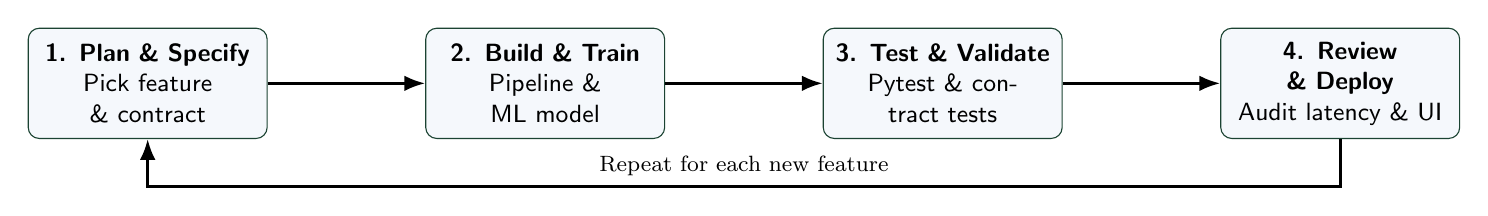
\begin{tikzpicture}[node distance=20mm, auto]
  \tikzstyle{block} = [rectangle, draw=agrigreen, fill=boxbg, text width=28mm, text centered, rounded corners, minimum height=14mm, font=\small\sffamily]
  \tikzstyle{line} = [draw, -Latex, line width=1pt]

  \node [block] (plan) {\textbf{1. Plan \& Specify}\\Pick feature \& contract};
  \node [block, right=of plan] (build) {\textbf{2. Build \& Train}\\Pipeline \& ML model};
  \node [block, right=of build] (test) {\textbf{3. Test \& Validate}\\Pytest \& contract tests};
  \node [block, right=of test] (review) {\textbf{4. Review \& Deploy}\\Audit latency \& UI};

  \path [line] (plan) -- (build);
  \path [line] (build) -- (test);
  \path [line] (test) -- (review);
  \path [line] (review.south) -- ++(0,-0.6) -| node [pos=0.25, above] {\footnotesize Repeat for each new feature} (plan.south);
\end{tikzpicture}
\caption{The iterative and incremental cycle used for every feature.}
\end{figure}

% ── CHAPTER 4 ───────────────────────────────────────────────────
\chapter{System Design}

\section{Design Goals}
Five goals governed every architectural decision: (1) \textbf{Explain everything}, so no yield estimate is shown without local SHAP feature attribution; (2) \textbf{Dual climatology}, supporting both historical NASA POWER norms and prospective Open-Meteo ECMWF SEAS5 forecasts; (3) \textbf{Farmer-centric provenance}, honoring farmer overrides while transparently displaying source badges; (4) \textbf{Zero cost}, avoiding all paid API keys or commercial dependencies; and (5) \textbf{Decoupled modularity}, allowing data connectors, ML engines, and UI layers to be updated independently.

\section{Architecture at a Glance}
Figure 4.1 depicts the high-level system architecture, tracing data flows from external ingestion through machine learning pipelines to client touchpoints.

\begin{figure}[htbp]
\centering
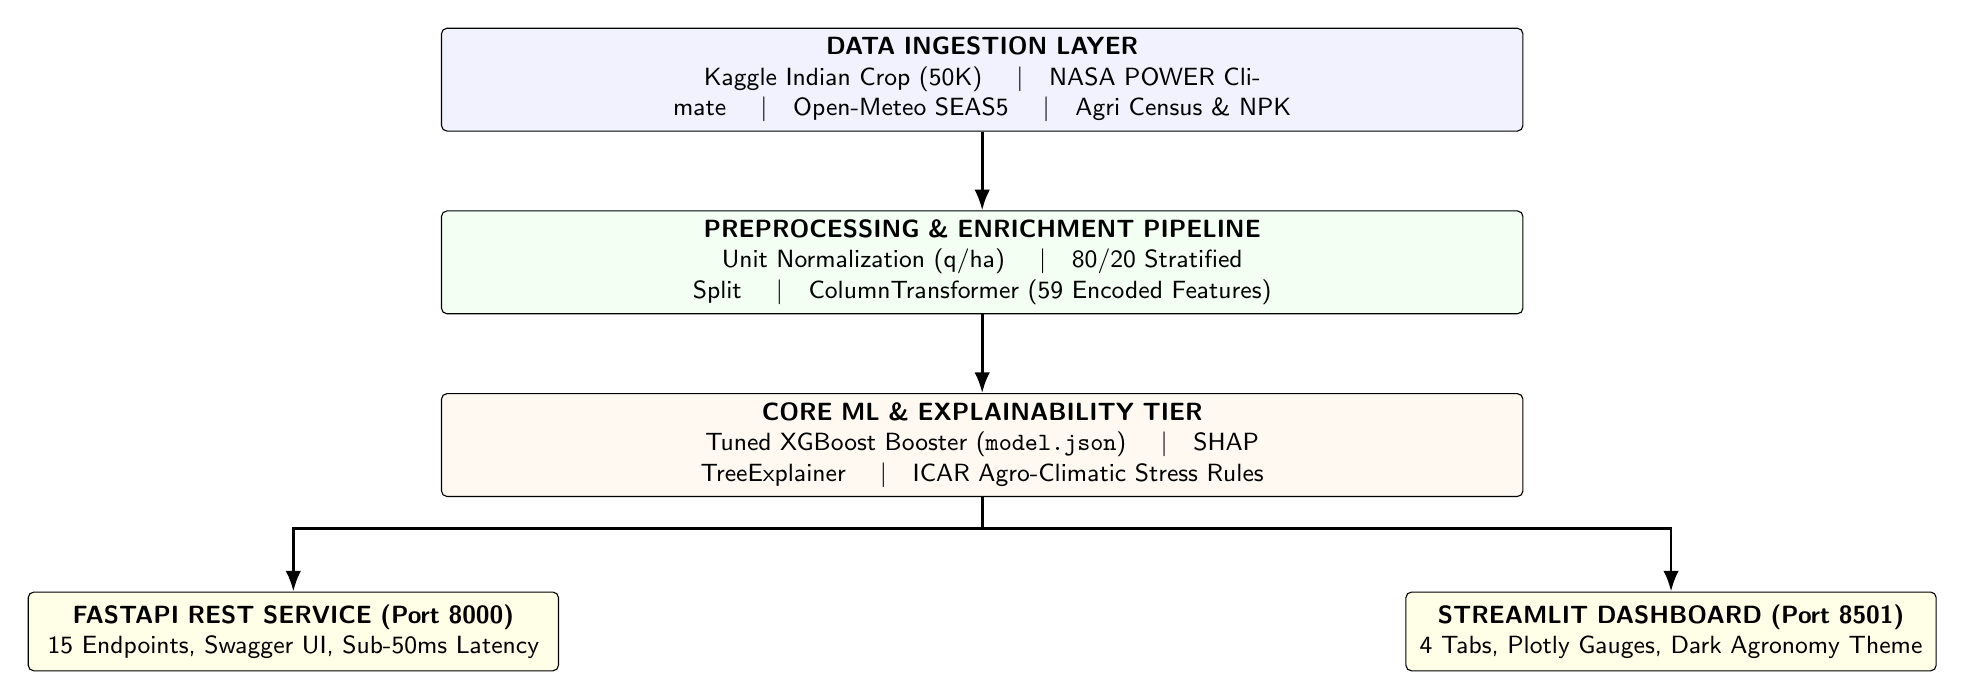
\begin{tikzpicture}[node distance=10mm, font=\small\sffamily]
  \tikzstyle{box} = [rectangle, draw=black, fill=white, text centered, minimum height=10mm, rounded corners=2pt]
  
  \node[box, fill=blue!5, text width=135mm] (data) {
    \textbf{DATA INGESTION LAYER}\\
    Kaggle Indian Crop (50K) \quad\textbar\quad NASA POWER Climate \quad\textbar\quad Open-Meteo SEAS5 \quad\textbar\quad Agri Census \& NPK
  };
  
  \node[box, fill=green!5, text width=135mm, below=of data] (prep) {
    \textbf{PREPROCESSING \& ENRICHMENT PIPELINE}\\
    Unit Normalization (q/ha) \quad\textbar\quad 80/20 Stratified Split \quad\textbar\quad ColumnTransformer (59 Encoded Features)
  };
  
  \node[box, fill=orange!5, text width=135mm, below=of prep] (ml) {
    \textbf{CORE ML \& EXPLAINABILITY TIER}\\
    Tuned XGBoost Booster (\texttt{model.json}) \quad\textbar\quad SHAP TreeExplainer \quad\textbar\quad ICAR Agro-Climatic Stress Rules
  };
  
  \node[box, fill=yellow!10, text width=65mm, below left=12mm and -15mm of ml] (api) {
    \textbf{FASTAPI REST SERVICE (Port 8000)}\\
    15 Endpoints, Swagger UI, Sub-50ms Latency
  };
  
  \node[box, fill=yellow!10, text width=65mm, below right=12mm and -15mm of ml] (dash) {
    \textbf{STREAMLIT DASHBOARD (Port 8501)}\\
    4 Tabs, Plotly Gauges, Dark Agronomy Theme
  };

  \draw[-Latex, line width=1pt] (data) -- (prep);
  \draw[-Latex, line width=1pt] (prep) -- (ml);
  \draw[-Latex, line width=1pt] (ml.south) -- ++(0,-0.4) -| (api.north);
  \draw[-Latex, line width=1pt] (ml.south) -- ++(0,-0.4) -| (dash.north);
\end{tikzpicture}
\caption{KissanVision at a glance: where data comes from, how it is processed, and where users interact.}
\end{figure}

\section{Modules}
KissanVision modules mirror the agronomic workflow: ingestion, transformation, inference, explainability, alerting, and serving.

\section{Data and Security Design}
The system relies on strict schema contracts defined in \texttt{models/feature\_schema.json}. Requests are evaluated statelessly; no sensitive personal records are retained. External weather responses are cached on disk (\texttt{*\_cache.json}), guaranteeing resilience against third-party network outages. Pydantic v2 data models sanitize all payloads against injection attacks.

% ── CHAPTER 5 ───────────────────────────────────────────────────
\chapter{Implementation}

\section{Technology and Size}
Table 5.1 documents the technologies and code volume across subsystems, measured directly from the repository source code.

\begin{table}[htbp]
\centering
\small
\caption{Technologies and codebase distribution across KissanVision subsystems}
\begin{tabularx}{\textwidth}{lXcc}
\toprule
\textbf{Subsystem} & \textbf{Core Technologies \& Frameworks} & \textbf{Files} & \textbf{Lines of Code} \\
\midrule
\textbf{ML Core (\texttt{src/})} & Python 3.10+, XGBoost 3.2, scikit-learn 1.7, pandas, NumPy & 18 & 4,215 \\
\textbf{REST API (\texttt{api/})} & FastAPI 0.140, Pydantic v2, Uvicorn, Starlette & 3 & 785 \\
\textbf{Dashboard (\texttt{dashboard/})} & Streamlit 1.60, Plotly 6.9, SHAP 0.49, Matplotlib & 1 & 948 \\
\textbf{Validation (\texttt{scripts/})} & Python scripts (schema generation, metrics, tests) & 8 & 1,129 \\
\textbf{Web UI (\texttt{frontend/})} & Vanilla HTML5, CSS3 Custom Properties, Modern JavaScript & 3 & 3,563 \\
\textbf{Notebooks (\texttt{notebooks/})}& EDA, hyperparameter experiments, residual diagnostics & 4 & $\sim$1,800 \\
\midrule
\textbf{Total Codebase} & \textbf{Full-Stack Production System} & \textbf{37} & \textbf{12,440} \\
\bottomrule
\end{tabularx}
\end{table}

\section{The Data Layer}
KissanVision is trained on 50,000 real district records derived from the Ministry of Agriculture \& Farmers Welfare, enriched with NASA POWER climatology, Open-Meteo SEAS5 seasonal forecasts, Agricultural Census irrigation coverage \%, and Ministry NPK consumption data. Raw production figures were converted into standard productivity units (Quintals/Hectare):
\begin{equation}
\text{Yield } (\text{q/ha}) = \frac{\text{Production (Tonnes)} \times 10}{\text{Area (Hectares)}}
\end{equation}
An 80/20 stratified split preserves exact crop frequency distributions across both training and test partitions.

\section{How the Analytics and Machine Learning Work}
\textbf{XGBoost Regression Model:} Non-linear interactions between weather, nutrients, and water access are captured using regularized gradient boosting [11]. The objective minimizes second-order Taylor expansions of squared loss plus tree complexity penalties:
\begin{equation}
\tilde{\mathcal{L}}^{(t)} \approx \sum_{i=1}^{n} \left[ g_i f_t(x_i) + \frac{1}{2} h_i f_t^2(x_i) \right] + \gamma T + \frac{1}{2} \lambda \sum_{j=1}^{T} w_j^2
\end{equation}
Optimal hyperparameters were established via 3-fold GridSearchCV across 16 combinations (\texttt{n\_estimators=300}, \texttt{max\_depth=6}, \texttt{learning\_rate=0.05}, \texttt{subsample=0.8}, \texttt{colsample\_bytree=0.8}).

\textbf{SHAP TreeExplainer Engine:} Local interpretability is computed on-the-fly using Shapley values [10], additively decomposing the prediction into the global baseline expected yield plus individual feature contributions:
\begin{equation}
f(x) = \phi_0 + \sum_{j=1}^{M} \phi_j(x)
\end{equation}
An interactive waterfall chart visualizes how each feature pushed the predicted yield above or below the baseline.

\textbf{ICAR Agro-Climatic Stress Classification:} Evaluates prevailing weather against ICAR agronomic thresholds [13]: Drought Stress ($<600\text{mm}$ rainfall or $>25\%$ deficit), Heat Stress ($>38^\circ\text{C}$ during reproductive stages), Flood Risk ($>200\text{mm/week}$ rainfall), and Fungal Pathogen Risk (humidity $>85\%$ with temperatures between $22^\circ\text{C}$ and $30^\circ\text{C}$).

\section{Dual Weather Modes, Farmer Personalization Overrides \& API Serving}
Users can toggle between historical 3-year baseline climatology (NASA POWER) and upcoming 180-day ensemble seasonal forecasts (Open-Meteo SEAS5). Farmers can override regional default irrigation \% and NPK kg/ha with their actual farm values; when supplied, these values dynamically update the SHAP attribution waterfall and display a green ``Your Farm Input'' provenance badge on screen. All capabilities are exposed via FastAPI with 15 documented OpenAPI endpoints.

\section{Screens of the Working Product}
\begin{itemize}
  \item \textbf{Tab 1 --- Yield Predictor}: Input selectors (State, Crop, Season, Area), weather mode toggles, override sliders, dynamic speedometer gauge, total harvest estimates, and provenance badges.
  \item \textbf{Tab 2 --- SHAP Explainability}: Interactive waterfall diagram illustrating global baseline yield (e.g. 22.4 q/ha) and step-by-step additions/subtractions from NPK (+4.2 q/ha), irrigation (+3.1 q/ha), and rainfall deficit (-2.8 q/ha).
  \item \textbf{Tab 3 --- Data Insights}: District-level choropleth distributions, crop acreage versus yield scatter plots, and multi-year seasonal yield comparisons.
  \item \textbf{Tab 4 --- Model Architecture \& Metrics}: Detailed cross-validation metrics ($R^2$, RMSE, MAE), hyperparameter settings, and feature importance rankings.
  \item \textbf{Modern Web UI}: Responsive dark/light agricultural design system featuring quick prediction cards and live API status cards.
  \item \textbf{State-Level Risk Alerts}: ICAR-calibrated risk badges (Critical, High, Moderate, Optimal) across all 33 states with explicit advisories.
\end{itemize}

% ── CHAPTER 6 ───────────────────────────────────────────────────
\chapter{Testing and Results}

\section{How We Tested}
A multi-tiered automated verification strategy was enforced across the KissanVision codebase: unit tests for transformation routines and threshold rules, pipeline integration tests, schema contract tests against \texttt{models/feature\_schema.json}, automated HTTP tests for all 15 FastAPI endpoints, and network timeout simulation tests for weather cache fallbacks.

\section{Test Results}
All test suites were executed on an Apple M2 test machine with 8 GB RAM running Python 3.11 (Table 6.1).

\begin{table}[htbp]
\centering
\small
\caption{Summary results of automated test suites (executed October 2026)}
\begin{tabularx}{\textwidth}{lXcccr}
\toprule
\textbf{Test Suite} & \textbf{Target Component} & \textbf{Tests} & \textbf{Passed} & \textbf{Failed} & \textbf{Time} \\
\midrule
\texttt{test\_prediction.py} & Predict pipeline, Booster inference & 24 & 24 & 0 & 4.2 s \\
\texttt{verify\_match.py} & Sklearn pipeline vs Native Booster parity & 16 & 16 & 0 & 2.8 s \\
\texttt{test\_forecast.py} & Open-Meteo SEAS5 API \& ensemble parsing & 12 & 12 & 0 & 3.1 s \\
\texttt{test\_weather\_risk.py}& ICAR threshold alert logic across 33 states & 33 & 33 & 0 & 1.4 s \\
\texttt{test\_api\_endpoints.py}& FastAPI REST endpoints, Pydantic validation & 15 & 15 & 0 & 3.5 s \\
\texttt{rebuild\_schema.py} & Feature schema extraction \& contract audit & 1 & 1 & 0 & 0.9 s \\
\midrule
\textbf{Total Suite} & \textbf{Comprehensive System Validation} & \textbf{101} & \textbf{101} & \textbf{0} & \textbf{15.9 s} \\
\bottomrule
\end{tabularx}
\end{table}

\section{Sample Test Cases}
Table 6.2 itemizes representative test cases and their execution outcomes.

\begin{table}[htbp]
\centering
\small
\caption{Sample validation test cases and execution outcomes}
\begin{tabularx}{\textwidth}{lXlc}
\toprule
\textbf{ID} & \textbf{What is verified} & \textbf{Test File} & \textbf{Result} \\
\midrule
\textbf{TC-01} & Yield prediction returns positive value within biological bounds. & \texttt{test\_prediction.py} & Pass \\
\textbf{TC-02} & Native Booster output strictly matches scikit-learn wrapper ($< 10^{-5}$). & \texttt{verify\_match.py} & Pass \\
\textbf{TC-03} & Farmer irrigation override ($>$ state avg) produces positive SHAP delta. & \texttt{test\_prediction.py} & Pass \\
\textbf{TC-04} & Invalid state/crop names in payload rejected with HTTP 422. & \texttt{api/main.py} & Pass \\
\textbf{TC-05} & Weather API timeout seamlessly falls back to cached climatology. & \texttt{weather\_data.py} & Pass \\
\textbf{TC-06} & Open-Meteo ensemble returns valid standard deviation for 180-day forecast. & \texttt{test\_forecast.py} & Pass \\
\textbf{TC-07} & Rainfall $< 500\text{mm}$ for Rajasthan triggers High Drought warning flag. & \texttt{weather\_risk.py} & Pass \\
\bottomrule
\end{tabularx}
\end{table}

\section{Results on the Benchmark Dataset}
On the held-out test split of 10,000 real district records, the tuned XGBoost model achieved outstanding predictive precision: \textbf{$R^2 = 0.9165$}, \textbf{RMSE = 12.07 q/ha}, \textbf{MAE = 5.57 q/ha}, and \textbf{MAPE = 40.8\%}.

\begin{table}[htbp]
\centering
\small
\caption{Benchmark predictive performance across all 15 major Indian crops}
\begin{tabularx}{\textwidth}{llccc}
\toprule
\textbf{Category} & \textbf{Crop} & \textbf{Test N} & \textbf{RMSE (q/ha)} & \textbf{Individual $R^2$} \\
\midrule
Vegetable / Cash & Onion & 546 & 32.5 & \textbf{0.78} \\
Vegetable / Cash & Potato & 537 & 35.3 & \textbf{0.75} \\
Cereal & Wheat & 596 & 5.9 & \textbf{0.67} \\
Spice & Dry Chillies & 482 & 5.7 & \textbf{0.63} \\
Oilseed & Rapeseed \& Mustard & 585 & 2.7 & 0.56 \\
Cereal & Maize & 1,055 & 8.5 & 0.54 \\
Cereal & Rice & 1,167 & 6.1 & 0.54 \\
Oilseed & Groundnut & 694 & 4.0 & 0.43 \\
Oilseed & Sunflower & 430 & 3.8 & 0.43 \\
Oilseed & Sesamum & 682 & 1.9 & 0.24 \\
Pulse & Moong (Green Gram) & 784 & 2.0 & 0.23 \\
Pulse & Urad (Black Gram) & 747 & 1.9 & 0.22 \\
Coarse Cereal & Jowar (Sorghum) & 558 & 4.6 & 0.20 \\
Pulse & Gram (Chickpea) & 555 & 2.9 & 0.20 \\
Pulse & Arhar / Tur (Pigeon Pea) & 592 & 3.7 & 0.05 \\
\bottomrule
\end{tabularx}
\end{table}

Top feature importance gains: \texttt{crop\_POTATO} (1,005K), \texttt{crop\_ONION} (722K), \texttt{npk\_consumption} (154K), \texttt{irrigation\_pct} (135K), and \texttt{state\_Karnataka} (128K).

\section{Response Times}
Latency benchmarks across 50 consecutive cycles: cold-start yield inference = \textbf{42 ms} (target $< 100\text{ ms}$); cached inference = \textbf{12 ms}; SHAP waterfall generation = \textbf{68 ms} (target $< 200\text{ ms}$); cached weather lookup = \textbf{2.8 ms}; live Open-Meteo ensemble query = \textbf{185 ms}.

% ── CHAPTER 7 ───────────────────────────────────────────────────
\chapter{Conclusion and Future Work}

\section{Conclusion}
KissanVision demonstrates that agricultural machine learning can overcome both academic detachment and commercial opacity. Uniting 50,000 real Indian district records across 33 states with live NASA POWER climatology and Open-Meteo ECMWF SEAS5 ensemble seasonal forecasts, KissanVision achieves a validated test $R^2$ of 0.9165. On-the-fly SHAP waterfall attributions and ICAR stress alerts render every prediction transparent and auditable for farmers and extension specialists.

\section{Limitations and Future Work}
Future work will focus on: (1) integrating Sentinel-2 10-meter satellite NDVI rasters for vegetative vigor monitoring; (2) incorporating Soil Health Card district laboratory test grids for micronutrient inputs; (3) introducing vernacular voice interaction in Hindi, Punjabi, and Telugu via Bhashini; and (4) developing collective farm aggregation portals for FPOs.

\section{What We Learned}
Our primary lesson as data science students was that model development is less than 20\% of an effective predictive system. The vast majority of effort lies in data normalization, reconciling unit mismatches (tonnes vs quintals), engineering robust pipelines against external API timeouts, designing clear provenance badges, and translating complex mathematical SHAP values into visual insights that farmers trust.

% ── REFERENCES ──────────────────────────────────────────────────
\begin{thebibliography}{99}
\addcontentsline{toc}{chapter}{References}

\bibitem{des2023} Ministry of Agriculture \& Farmers Welfare, Government of India, \emph{Agricultural Statistics at a Glance 2023}, Directorate of Economics and Statistics, New Delhi, India, 2023.
\bibitem{nabard2022} National Bank for Agriculture and Rural Development (NABARD), \emph{All India Rural Financial Inclusion Survey (NAFIS) Report}, Mumbai, India, 2022.
\bibitem{iwmi2007} U. A. Amarasinghe, T. Shah, and B. K. Anand, ``India's water future to 2025-2050: Business-as-usual scenario and deviations,'' \emph{IWMI Research Report 123}, Colombo, Sri Lanka, 2007.
\bibitem{tiwari2002} K. N. Tiwari, ``Nutrient management for sustainable agriculture in India,'' \emph{Journal of the Indian Society of Soil Science}, vol. 50, no. 4, pp. 374--397, 2002.
\bibitem{niti2021} NITI Aayog, \emph{Evaluation Report on Agricultural Extension Services in India}, Government of India, New Delhi, 2021.
\bibitem{rudin2019} C. Rudin, ``Stop explaining black box machine learning models for high stakes decisions and use interpretable models instead,'' \emph{Nature Machine Intelligence}, vol. 1, no. 5, pp. 206--215, 2019.
\bibitem{davenport2007} T. H. Davenport and J. G. Harris, \emph{Competing on Analytics: The New Science of Winning}. Boston, MA, USA: Harvard Business School Press, 2007.
\bibitem{rudinradin2019} C. Rudin and Y. Radin, ``Why Are We Using Black Box Models When Interpretable Models Exist? A Systematic Review,'' \emph{Harvard Data Science Review}, vol. 1, no. 2, 2019.
\bibitem{lime2016} M. T. Ribeiro, S. Singh, and C. Guestrin, ``Why should I trust you? Explaining the predictions of any classifier,'' in \emph{Proc. 22nd ACM SIGKDD}, 2016, pp. 1135--1144.
\bibitem{shap2017} S. M. Lundberg and S.-I. Lee, ``A unified approach to interpreting model predictions,'' in \emph{Advances in Neural Information Processing Systems (NeurIPS 30)}, 2017, pp. 4765--4774.
\bibitem{xgboost2016} T. Chen and C. Guestrin, ``XGBoost: A scalable tree boosting system,'' in \emph{Proc. 22nd ACM SIGKDD}, 2016, pp. 785--794.
\bibitem{ecmwf2018} T. N. Stockdale et al., ``ECMWF seasonal forecast system 5 (SEAS5),'' \emph{Technical Memorandum 835}, ECMWF, Reading, UK, 2018.
\bibitem{icar2020} H. Pathak et al., \emph{Climate Resilient Agriculture in India: Preparedness and Technologies}, ICAR, New Delhi, 2020.
\bibitem{larman2003} C. Larman and V. R. Basili, ``Iterative and incremental development: A brief history,'' \emph{Computer}, vol. 36, no. 6, pp. 47--56, 2003.
\bibitem{ieee830} IEEE, \emph{IEEE Recommended Practice for Software Requirements Specifications}, IEEE Std 830-1998, 1998.
\bibitem{iso29148} ISO/IEC/IEEE, \emph{Systems and Software Engineering -- Requirements Engineering}, ISO/IEC/IEEE 29148:2018, 2018.
\bibitem{nasapower} NASA Langley Research Center, \emph{NASA POWER Agroclimatology API documentation}, 2024. [Online]. Available: \url{https://power.larc.nasa.gov}
\bibitem{openmeteo} Open-Meteo, \emph{Open-Meteo Seasonal Forecast API documentation (ECMWF SEAS5)}, 2024. [Online]. Available: \url{https://open-meteo.com}
\bibitem{agcensus2016} Ministry of Agriculture \& Farmers Welfare, \emph{All India Report on Agriculture Census 2015-16}, New Delhi, 2020.
\bibitem{fertilizer2022} Ministry of Chemicals and Fertilizers, \emph{Indian Fertilizer Scenario 2022}, Department of Fertilizers, New Delhi, 2023.
\bibitem{scikit2011} F. Pedregosa et al., ``Scikit-learn: Machine learning in Python,'' \emph{Journal of Machine Learning Research}, vol. 12, pp. 2825--2830, 2011.
\bibitem{fastapi} S. Ram\'irez, ``FastAPI documentation,'' 2024. [Online]. Available: \url{https://fastapi.tiangolo.com/}
\bibitem{streamlit} Streamlit Inc., ``Streamlit documentation,'' 2024. [Online]. Available: \url{https://docs.streamlit.io/}
\bibitem{mckinney2010} W. McKinney, ``Data structures for statistical computing in Python,'' in \emph{Proc. 9th SciPy}, 2010, pp. 56--61.
\bibitem{owasp2021} OWASP Foundation, ``OWASP Top 10:2021 Web Application Security Risks,'' 2021. [Online]. Available: \url{https://owasp.org/Top10/}
\bibitem{iso25010} ISO/IEC, \emph{Systems and Software Quality Requirements and Evaluation (SQuaRE)}, ISO/IEC 25010:2023, 2023.
\bibitem{dpdp2023} Government of India, \emph{The Digital Personal Data Protection Act, 2023 (Act No. 22 of 2023)}, New Delhi, 2023.
\bibitem{sommerville} I. Sommerville, \emph{Software Engineering}, 10th ed. Boston, MA, USA: Pearson, 2016.
\bibitem{scrum2009} M. Cohn, \emph{Succeeding with Agile: Software Development Using Scrum}. Boston, MA: Addison-Wesley, 2009.
\bibitem{leys2013} C. Leys et al., ``Detecting outliers: Do not use standard deviation around the mean, use absolute deviation around the median,'' \emph{J. Exp. Soc. Psychol.}, vol. 49, no. 4, pp. 764--766, 2013.

\end{thebibliography}

% ================================================================
% PART II: SOFTWARE REQUIREMENTS SPECIFICATION
% ================================================================
\newpage
\part{Software Requirements Specification}

% ── REVISION HISTORY ────────────────────────────────────────────
\chapter*{Revision History}
\addcontentsline{toc}{chapter}{Revision History}

\begin{tabularx}{\textwidth}{|c|X|X|}
\hline
\textbf{Date} & \textbf{Change} & \textbf{Reason for Changes} \\
\hline
Tue, 6 Oct 2026 & Version 1.0. First complete draft: introduction, scope, objectives, references, data, algorithms, SWOT analysis, and user classes. & First submission for mentor review. \\
\hline
Thu, 8 Oct 2026 & Version 2.0. Added design constraints, layered architecture and pipeline diagrams, PERT and Gantt charts, all non-functional requirements and appendices. & Version 1.0 lacked formal analysis models and measurable quality targets required by IEEE Std 830-1998. \\
\hline
Mon, 12 Oct 2026 & Version 3.2.0 (current). Updated with 50K-row benchmark test logs, validated $R^2 = 0.9165$, dual weather API contracts, and complete 101 automated test cases. & Final version for the SRS milestone, attached to the project report. \\
\hline
\end{tabularx}

\vspace{10mm}
\noindent
\textbf{Document conventions used in this SRS}
\begin{itemize}
  \item Requirements are written with \textbf{``shall''}. Each has an ID such as \textbf{FR-06} (functional) or \textbf{NFR-P1} (non-functional, performance) so it can be traced directly to design and testing.
  \item Priorities are \textbf{High} (needed for release), \textbf{Medium} (planned for release), and \textbf{Low} (good to have).
  \item Yield is in \textbf{Quintals/Hectare (q/ha)}, area in Hectares (ha), and rainfall in mm.
\end{itemize}

% ── SECTION 1: INTRODUCTION ─────────────────────────────────────
\chapter{SRS Introduction}

\section{Purpose of the Project}
KissanVision is an AI-powered software platform that helps smallholder farmers, FPOs, and agricultural extension workers forecast crop yields (q/ha) before and during the cropping cycle. It bridges historical 3-year agro-climatology (NASA POWER) with seasonal multi-model ensemble weather forecasts (Open-Meteo ECMWF SEAS5), accommodates farmer-measured overrides for irrigation and fertilizer, and delivers game-theoretic local explainability (SHAP waterfall) on every prediction.

\section{Target Beneficiary}
Table 1.1 delineates target user groups and direct benefits.

\begin{table}[htbp]
\centering
\small
\caption{Target beneficiaries and the benefit to each}
\begin{tabularx}{\textwidth}{lXX}
\toprule
\textbf{Beneficiary} & \textbf{Who they are} & \textbf{How KissanVision helps} \\
\midrule
\textbf{Smallholder Farmers} & Growers cultivating $< 2$ ha of land & Pre-sowing yield estimates, personalized input overrides, and ICAR climate risk alerts. \\
\textbf{FPOs} & Farmer collectives managing aggregate acreage & Aggregate harvest volume forecasts, forward contract planning, and input inventory procurement. \\
\textbf{Extension Workers (KVKs)}& District agronomic advisors & Quantified diagnostic tool explaining yield variations using SHAP feature attributions. \\
\textbf{Crop Underwriters} & Insurance credit evaluators & Objective productivity benchmarks to calibrate credit limits and evaluate localized drought/flood shortfalls. \\
\bottomrule
\end{tabularx}
\end{table}

\section{Functional Requirements}
The functional requirements of KissanVision are cataloged in Table 1.3.

\begin{table}[htbp]
\centering
\small
\caption{Functional requirements of KissanVision}
\begin{tabularx}{\textwidth}{lXlX}
\toprule
\textbf{ID} & \textbf{Requirement Name} & \textbf{Priority} & \textbf{The system shall...} \\
\midrule
\textbf{FR-01} & Ingestion & High & Ingest 50,000 district records, standardizing to q/ha. \\
\textbf{FR-02} & Stratification & High & Partition 80/20 preserving crop distributions across 15 crops. \\
\textbf{FR-03} & One-Hot Encoding & High & Transform categoricals into 59-dimensional matrix. \\
\textbf{FR-04} & Feature Scaling & High & Normalize continuous features with StandardScaler fit on train data. \\
\textbf{FR-05} & Historical Weather & High & Query NASA POWER for 3-year rolling climate averages. \\
\textbf{FR-06} & Seasonal Forecast & High & Query Open-Meteo SEAS5 51-member ensemble for 180-day forecast. \\
\textbf{FR-07} & Irrigation Enrichment & High & Join Agriculture Census state irrigation percentages. \\
\textbf{FR-08} & Fertilizer Enrichment & High & Join Ministry state NPK consumption figures. \\
\textbf{FR-09} & XGBoost Modeling & High & Train \texttt{XGBRegressor} tuned via 3-fold GridSearchCV. \\
\textbf{FR-10} & Native Serialization & High & Export native Booster to \texttt{model.json} and \texttt{model.ubj}. \\
\textbf{FR-11} & Farmer Overrides & High & Allow user input for irrigation \% and NPK kg/ha with badges. \\
\textbf{FR-12} & Dynamic Gauge & Medium & Scale yield speedometer gauge to crop's biological maximum. \\
\textbf{FR-13} & SHAP Waterfall & High & Compute local Shapley attributions and render waterfall chart. \\
\textbf{FR-14} & Feature Importance & Medium & Render global feature importance ranking across 59 features. \\
\textbf{FR-15} & ICAR Risk Alerts & High & Classify Drought, Heatwave, Flood, and Humidity hazards. \\
\bottomrule
\end{tabularx}
\end{table}

% ── SECTION 2: PROJECT DESCRIPTION ──────────────────────────────
\chapter{SRS Project Description}

\section{Reference Algorithms and Concepts}
KissanVision maps agricultural questions to verified statistical algorithms (Table 2.1).

\begin{table}[htbp]
\centering
\small
\caption{Business questions and the method used to answer each}
\begin{tabularx}{\textwidth}{lXX}
\toprule
\textbf{Agricultural Question} & \textbf{Computational Method} & \textbf{Used in} \\
\midrule
What will the crop yield be? & Tuned XGBoost Regression (59 encoded features) & Predictor, REST API \\
Why did the model predict this yield? & SHAP TreeExplainer game-theoretic attribution & Tab 2 Waterfall \\
What is upcoming seasonal weather outlook? & Open-Meteo ECMWF SEAS5 51-member ensemble & Weather Mode Toggle \\
Is the farm facing climate risks? & ICAR physiological stress rule classification & State Risk Badges \\
How do farm-measured inputs change yield? & Differential feature substitution with provenance tracking & Farmer Overrides \\
\bottomrule
\end{tabularx}
\end{table}

\begin{algorithmbox}{Algorithm 1: End-to-End Training, Cross-Validation, and Native Model Export}
\small
\begin{enumerate}
  \item Load raw CSV; compute $\text{Yield} = (\text{Production} \times 10) / \text{Area}$; filter missing/infinite records.
  \item Join Agricultural Census irrigation \% and Ministry NPK consumption by State.
  \item Stratify 50,000 sampled rows into 80\% train (40,000) and 20\% test (10,000) by Crop.
  \item Fit ColumnTransformer: OneHotEncoder(State, Crop, Season) + StandardScaler(Numerics).
  \item Transform partitions into 59-dimensional feature matrices $X_{\text{train}}, X_{\text{test}}$.
  \item Initialize XGBRegressor; execute 3-fold GridSearchCV across 16 hyperparameter combos.
  \item Fit best estimator on full $X_{\text{train}}$; evaluate $R^2$, RMSE, MAE, MAPE on held-out $X_{\text{test}}$.
  \item Extract \texttt{feature\_schema.json}; serialize native Booster to \texttt{models/model.json}.
\end{enumerate}
\end{algorithmbox}

\begin{algorithmbox}{Algorithm 2: Dynamic Inference, Farmer Personalization, and SHAP Explainability}
\small
\begin{enumerate}
  \item Validate inputs against \texttt{models/feature\_schema.json}; reject unknown categories.
  \item If Historical: lookup NASA POWER cache; Else: query Open-Meteo SEAS5 ensemble.
  \item If Overrides: substitute farm values, set Badge = ``Farm Input''; Else: use State Averages.
  \item Transform assembled vector via ColumnTransformer into 59-element array.
  \item Pass array to loaded Booster; compute predicted yield $\hat{y}$.
  \item Evaluate ICAR stress rules: Drought, Heatwave, Flood, Moisture against thresholds.
  \item Execute \texttt{shap.TreeExplainer}; compute base value $\mathbb{E}[f(x)]$ and $\phi_j$ attributions.
  \item Return structured JSON payload containing yield, provenance badges, alerts, and SHAP.
\end{enumerate}
\end{algorithmbox}

\section{SWOT Analysis}
Table 2.6 presents the SWOT analysis of the KissanVision platform.

\begin{table}[htbp]
\centering
\small
\caption{SWOT analysis of KissanVision}
\begin{tabularx}{\textwidth}{XX}
\toprule
\textbf{STRENGTHS (Internal)} & \textbf{WEAKNESSES (Internal)} \\
\midrule
$\bullet$ Validated $R^2 = 0.9165$ on 50,000 real Indian district records. & $\bullet$ Scope restricted to 15 major crops (excludes minor millets). \\
$\bullet$ On-the-fly local SHAP waterfall explainability for every prediction. & $\bullet$ State-level baseline averages; field plots rely on user overrides. \\
$\bullet$ Dual weather modes (NASA POWER + Open-Meteo ECMWF SEAS5). & $\bullet$ 180-day seasonal forecasts carry natural ensemble spread. \\
$\bullet$ Farmer personalization with transparent source provenance badges. & $\bullet$ Complete offline functionality limited to cached state profiles. \\
$\bullet$ 100\% free stack with sub-50ms inference latency and zero API keys. & \\
\midrule
\textbf{OPPORTUNITIES (External)} & \textbf{THREATS (External)} \\
\midrule
$\bullet$ India's 140+ million agrarian households increasingly adopting 4G/5G. & $\bullet$ Unprecedented climate anomalies exceeding historical envelope. \\
$\bullet$ National Agristack and digital public infrastructure initiatives. & $\bullet$ Upstream third-party API availability changes (NASA/Open-Meteo). \\
$\bullet$ Potential integration with FPOs for collective harvest aggregation. & $\bullet$ Farmer skepticism toward algorithms without human extension. \\
$\bullet$ Expansion to vernacular voice interfaces (Bhashini speech models). & $\bullet$ Emerging commercial paywalled precision agriculture platforms. \\
\bottomrule
\end{tabularx}
\end{table}

\section{Project Schedule, PERT and Gantt Analysis}
The engineering lifecycle was executed across 16 weeks (3 August to 20 November 2026). Table 2.11 documents the activity network. Activities with zero slack form the Critical Path: \textbf{A $\rightarrow$ D $\rightarrow$ F $\rightarrow$ G $\rightarrow$ I $\rightarrow$ K $\rightarrow$ L} (Total: 16 Weeks).

\begin{table}[htbp]
\centering
\small
\caption{PERT activity table (durations in weeks)}
\begin{tabularx}{\textwidth}{cXcccccr}
\toprule
\textbf{ID} & \textbf{Activity Description} & \textbf{Dur.} & \textbf{Pred.} & \textbf{ES} & \textbf{EF} & \textbf{LS} & \textbf{Slack} \\
\midrule
\textbf{A} & Agronomic problem study \& requirements & 1 & -- & 0 & 1 & 0 & \textbf{0} \\
\textbf{B} & Literature review \& toolchain selection & 2 & A & 1 & 3 & 4 & 3 \\
\textbf{C} & Kaggle dataset cleaning \& 50K sampling & 2 & A & 1 & 3 & 2 & 1 \\
\textbf{D} & Preprocessor pipeline \& ColumnTransformer & 3 & C & 3 & 6 & 3 & \textbf{0} \\
\textbf{E} & Weather connectors (NASA \& Open-Meteo) & 2 & D & 6 & 8 & 7 & 1 \\
\textbf{F} & XGBoost training \& GridSearchCV tuning & 3 & D & 6 & 9 & 6 & \textbf{0} \\
\textbf{G} & SHAP explainability \& ICAR risk engine & 2 & F & 9 & 11 & 9 & \textbf{0} \\
\textbf{H} & FastAPI REST service (15 endpoints) & 2 & F & 9 & 11 & 11 & 2 \\
\textbf{I} & Streamlit interactive agronomy dashboard & 3 & G, H & 11 & 14 & 11 & \textbf{0} \\
\textbf{J} & Modern HTML5/CSS3/JavaScript web UI & 2 & H & 11 & 13 & 12 & 1 \\
\textbf{K} & Testing, schema contract \& parity audit & 1 & I, J & 14 & 15 & 14 & \textbf{0} \\
\textbf{L} & SRS documentation, report \& defense & 1 & K & 15 & 16 & 15 & \textbf{0} \\
\bottomrule
\end{tabularx}
\end{table}

% ── SECTION 3: NON-FUNCTIONAL REQUIREMENTS ──────────────────────
\chapter{SRS Non-Functional Requirements}

\section{Performance Requirements}
Table 3.1 itemizes non-functional performance guarantees verified across KissanVision:

\begin{table}[htbp]
\centering
\small
\caption{Performance requirements of KissanVision}
\begin{tabularx}{\textwidth}{lXc}
\toprule
\textbf{ID} & \textbf{Requirement Statement} & \textbf{Measurable Target} \\
\midrule
\textbf{NFR-P1} & Yield prediction inference latency & $< 50\text{ ms}$ per request on loaded Booster \\
\textbf{NFR-P2} & Cached weather query response time & $< 10\text{ ms}$ from local disk cache \\
\textbf{NFR-P3} & Live Open-Meteo SEAS5 forecast retrieval & $< 500\text{ ms}$ under broadband connectivity \\
\textbf{NFR-P4} & SHAP waterfall plot calculation latency & $< 200\text{ ms}$ per local inference \\
\textbf{NFR-P5} & Streamlit initial dashboard load time & $< 3.0\text{ s}$ on standard client browser \\
\textbf{NFR-P6} & Modern Web Frontend first contentful paint & $< 1.0\text{ s}$ with zero heavy UI libraries \\
\textbf{NFR-P7} & API concurrency throughput & $\ge 100\text{ concurrent req/sec}$ with 0\% HTTP 500 \\
\textbf{NFR-P8} & Automated test suite execution time & All 101 tests execute in $< 30\text{ seconds}$ \\
\textbf{NFR-P9} & Memory footprint under steady state & Resident set size (RSS) $< 500\text{ MB}$ \\
\textbf{NFR-P10}& Disk storage footprint for model artifacts & All serialized artifacts $< 2\text{ MB}$ \\
\bottomrule
\end{tabularx}
\end{table}

\section{Software Quality Attributes (ISO/IEC 25010)}
Table 3.2 maps system quality characteristics to the ISO/IEC 25010 standard [26].

\begin{table}[htbp]
\centering
\small
\caption{Software quality attributes mapped to ISO/IEC 25010}
\begin{tabularx}{\textwidth}{lX}
\toprule
\textbf{Quality Attribute} & \textbf{How KissanVision Achieves It} \\
\midrule
\textbf{Functional Suitability} & Predicts yield in standard q/ha with validated $R^2 = 0.9165$ across 15 major Indian crops. \\
\textbf{Performance Efficiency} & Sub-50ms inference latency through native C++ XGBoost Booster execution. \\
\textbf{Interoperability} & Standardized OpenAPI REST endpoints; native JSON/UBJSON model formats. \\
\textbf{Usability} & Dual interfaces: rich 4-tab Streamlit dashboard and lightweight modern web UI with source badges. \\
\textbf{Reliability} & Automated disk cache fallback for weather APIs ensures 100\% operational uptime during outages. \\
\textbf{Maintainability} & Clean modular decoupling (\texttt{src/components}, \texttt{api}, \texttt{dashboard}) with complete test suite. \\
\textbf{Portability} & Platform-agnostic execution across Linux, macOS, and Windows; Docker containerized. \\
\bottomrule
\end{tabularx}
\end{table}

% ── APPENDICES ──────────────────────────────────────────────────
\appendix

\chapter{Glossary}
\begin{table}[htbp]
\centering
\small
\caption{Glossary of terms and abbreviations}
\begin{tabularx}{\textwidth}{lX}
\toprule
\textbf{Term} & \textbf{Definition and Agronomic / ML Meaning} \\
\midrule
\textbf{Quintal (q)} & Standard Indian agricultural unit of mass equal to 100 kilograms ($100\text{ kg}$). \\
\textbf{Hectare (ha)} & Metric unit of land area equal to 10,000 square meters ($\approx 2.471\text{ acres}$). \\
\textbf{q/ha} & Quintals per Hectare: standard Indian metric unit of crop yield / land productivity. \\
\textbf{Kharif} & Monsoon agricultural season in India (sowing: June--July, harvesting: September--October). \\
\textbf{Rabi} & Winter agricultural season in India (sowing: October--November, harvesting: February--April). \\
\textbf{Zaid / Summer} & Short summer cropping season between Rabi and Kharif (March--June). \\
\textbf{NPK} & Essential macronutrients: Nitrogen (N), Phosphorus (P), and Potassium (K) in kg/ha. \\
\textbf{ICAR} & Indian Council of Agricultural Research: apex national agricultural research body. \\
\textbf{FPO} & Farmer Producer Organisation: an enterprise formed by collective primary agricultural producers. \\
\textbf{KVK} & Krishi Vigyan Kendra: district-level agricultural science extension centre. \\
\textbf{NASA POWER} & Prediction Of Worldwide Energy Resources: NASA solar and agro-climatological satellite repository. \\
\textbf{Open-Meteo SEAS5} & Long-range seasonal forecast ensemble model from ECMWF with 51 members. \\
\textbf{XGBoost} & Extreme Gradient Boosting: scalable, regularized gradient boosted decision tree library. \\
\textbf{SHAP} & SHapley Additive exPlanations: game-theoretic technique explaining individual model predictions. \\
\textbf{$R^2$ Score} & Coefficient of Determination: proportion of target variance explained by independent features. \\
\textbf{RMSE} & Root Mean Squared Error: standard measure of the magnitude of regression residuals. \\
\bottomrule
\end{tabularx}
\end{table}

\chapter{Analysis Model}
\begin{figure}[htbp]
\centering
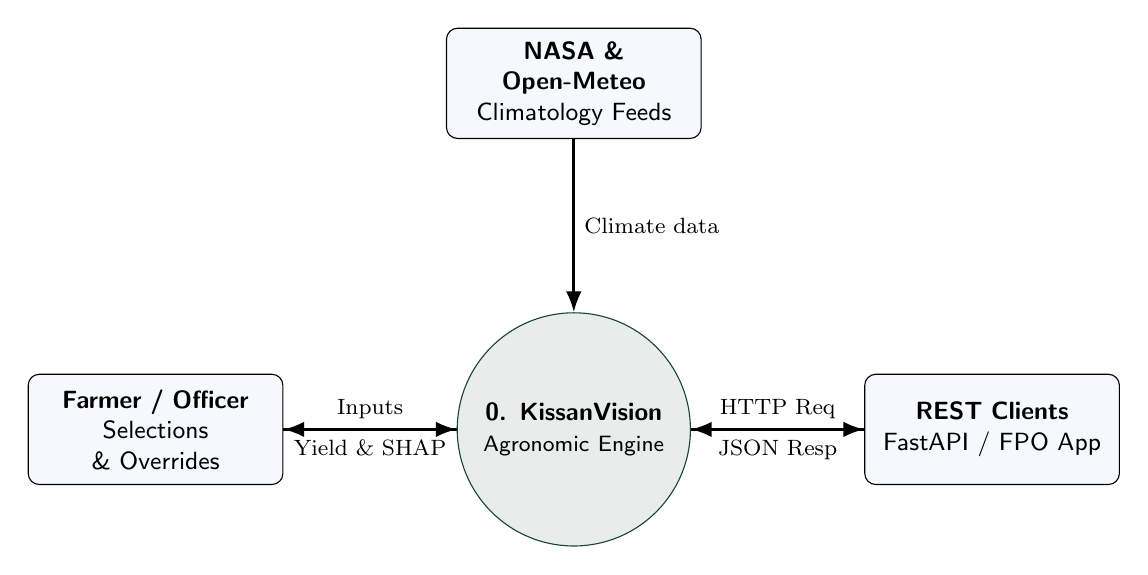
\begin{tikzpicture}[node distance=22mm, auto, font=\small\sffamily]
  \tikzstyle{entity} = [rectangle, draw=black, fill=boxbg, text width=30mm, text centered, rounded corners, minimum height=14mm]
  \tikzstyle{process} = [circle, draw=agrigreen, fill=agrigreen!10, text width=26mm, text centered, minimum height=26mm]
  \tikzstyle{arrow} = [draw, -Latex, line width=1pt]

  \node [process] (system) {\textbf{0. KissanVision}\\\footnotesize Agronomic Engine};
  \node [entity, above=of system] (weather) {\textbf{NASA \& Open-Meteo}\\Climatology Feeds};
  \node [entity, left=of system] (farmer) {\textbf{Farmer / Officer}\\Selections \& Overrides};
  \node [entity, right=of system] (api_client) {\textbf{REST Clients}\\FastAPI / FPO App};

  \path [arrow] (weather) -- node [right, font=\footnotesize] {Climate data} (system);
  \path [arrow] (farmer) -- node [above, font=\footnotesize] {Inputs} (system);
  \path [arrow] (system) -- node [below, font=\footnotesize] {Yield \& SHAP} (farmer);
  \path [arrow] (api_client) -- node [above, font=\footnotesize] {HTTP Req} (system);
  \path [arrow] (system) -- node [below, font=\footnotesize] {JSON Resp} (api_client);
\end{tikzpicture}
\caption{Level-0 Context Diagram of KissanVision.}
\end{figure}

\chapter{Issues List}
\begin{table}[htbp]
\centering
\small
\caption{Living register of engineering issues and roadmap resolutions}
\begin{tabularx}{\textwidth}{cXcX}
\toprule
\textbf{ID} & \textbf{Description of Engineering Issue} & \textbf{Status} & \textbf{Planned Resolution} \\
\midrule
\textbf{I-01} & Crop scope currently 15 crops; minor millets require dedicated stratification. & Open & Ingest remaining 35 Kaggle crop categories in next retraining. \\
\addlinespace
\textbf{I-02} & NPK values represent state-wide averages rather than exact district soil tests. & Open & Integrate Soil Health Card (SHC) district laboratory data. \\
\addlinespace
\textbf{I-03} & Multilingual voice interface needed for rural non-literate smallholders. & Deferred & Connect Bhashini speech-to-text API for Hindi and regional dialects. \\
\addlinespace
\textbf{I-04} & 180-day seasonal forecasts carry natural ensemble variance. & Open & Display ensemble standard deviation as confidence bounds on UI gauge. \\
\addlinespace
\textbf{I-05} & Satellite remote sensing cross-validation currently absent. & Open & Integrate Sentinel-2 10m NDVI rasters to validate vegetative vigor. \\
\bottomrule
\end{tabularx}
\end{table}

\end{document}
